% This is samplepaper.tex, a sample chapter demonstrating the
% LLNCS macro package for Springer Computer Science proceedings;
% Version 2.21 of 2022/01/12
%
\documentclass[runningheads]{llncs}
%
\usepackage[T1]{fontenc}
% T1 fonts will be used to generate the final print and online PDFs,
% so please use T1 fonts in your manuscript whenever possible.
% Other font encondings may result in incorrect characters.
%
\usepackage{graphicx}
% Used for displaying a sample figure. If possible, figure files should
% be included in EPS format.
%
% If you use the hyperref package, please uncomment the following two lines
% to display URLs in blue roman font according to Springer's eBook style:
%\usepackage{color}
%\renewcommand\UrlFont{\color{blue}\rmfamily}
\usepackage[dvipsnames]{xcolor}
\usepackage{xparse}
\usepackage[hidelinks]{hyperref}
\usepackage[inline]{enumitem}
\newenvironment{inlinelist}{\begin{enumerate*}[label=\emph{(\roman*)}]}{\end{enumerate*}}
\usepackage{acronym}
\usepackage[firstpage]{draftwatermark}

\acrodef{ABMS}{Agent-Based Modelling and Simulation}
\acrodef{API}{Application Programming Interface}
\acrodef{CAS}{Collective Adaptive System}
\acrodef{FFI}{Foreign Function Interface}
\acrodef{HIL}{Hardware-in-the-Loop}
\acrodef{IDL}{Interface Description Langage}
\acrodef{IoT}{Internet of Things}
\acrodef{JVM}{Java Virtual Machine}
\acrodef{JS}{JavaScript}
\acrodef{ODD}{Overview, Design concepts, and Details}
\acrodef{WASM}{WebAssembly}
\acrodef{ECS}{Entity Component System}
\acrodef{DOTS}{Data-Oriented Technology Stack}


%%%%%% LISTINGS
\usepackage{listings}

\lstdefinelanguage{Kotlin}{
    comment=[l]{//},
    emph={delegate, filter, filterIsInstance, flatMap, toSet, firstOrNull, forEach, lazy, map, mapNotNull, println, return@, sequence, yield, Array, Byte, Double, Float, Int, Iterable, Long, Runnable, Short, String},
    keywords={operator, infix, init, abstract, actual, as, as?, break, by, class, companion, continue, data, do, dynamic, else, enum, expect, false, final, for, fun, get, if, import, in, interface, internal, is, null, object, override, package, private, public, return, set, super, suspend, this, throw, true, try, typealias, val, var, vararg, when, where, while, it},
    morecomment=[s]{/*}{*/},
    morestring=[b]",
    morestring=[s]{"""*}{*"""},
    ndkeywords={@Deprecated, @JvmField, @JvmName, @JvmOverloads, @JvmStatic, @JvmSynthetic},
    sensitive=true,
}

\usepackage[most]{tcolorbox}

% Toggle: comment/uncomment as needed
\newif\iftodos
\todostrue      % show todos
% \todofalse    % hide todos

% Colors (pick any you like)
\definecolor{FilippoC}{HTML}{1F77B4}
\definecolor{DaniloC}{HTML}{D62728}
\definecolor{AngelaC}{HTML}{2CA02C}
\definecolor{MartinaC}{HTML}{9467BD}

% Base inline box macro: label, color, text
\newcommand{\pnote}[3]{%
    \iftodos
    \tcbox[
        on line,
        boxsep=1.2pt,
        left=3pt,right=3pt,top=1.2pt,bottom=1.2pt,
        colback=#2!10,
        colframe=#2!65!black,
        arc=2pt,
        boxrule=0.6pt
    ]{\textsf{\bfseries #1:}~#3}%
    \else
    \ignorespaces
    \fi
}

% Per-person commands
\newcommand{\filippo}[1]{\pnote{Filippo}{FilippoC}{#1}}
\newcommand{\danilo}[1]{\pnote{Danilo}{DaniloC}{#1}}
\newcommand{\angela}[1]{\pnote{Angela}{AngelaC}{#1}}
\newcommand{\martina}[1]{\pnote{Martina}{MartinaC}{#1}}
\usepackage{cleveref}
%

\NewDocumentCommand{\CommentBox}{m m m}{%
  \begin{tcolorbox}[
    enhanced,
    breakable,
    colback=#1!30,
    colframe=#1!90!black,
    coltitle=black,
    title={#2:},
    fonttitle=\bfseries,
    boxrule=0.8pt,
    arc=2mm,
    left=1.5mm,right=1.5mm,top=1mm,bottom=1mm,
    attach title to upper,
  ]
  ~#3
  \end{tcolorbox}
}

\makeatletter
\AtBeginDocument
 {
   \def\ltx@label#1{\cref@label{#1}}%add braces
   \def\label@in@display@noarg#1{\cref@old@label@in@display{#1}}%remove braces
\def\label@in@mmeasure@noarg#1{%
    \begingroup%
      \measuring@false%
      \cref@old@label@in@display{#1}%remove braces for multline, see https://tex.stackexchange.com/q/737204/2388
    \endgroup}%
 } %
\makeatother

% Author-specific commands (choose any colors you like)
\NewDocumentCommand{\Danilo}{m}{\CommentBox{RoyalBlue}{Danilo}{#1}}
\NewDocumentCommand{\Martina}{m}{\CommentBox{ForestGreen}{Martina}{#1}}
\NewDocumentCommand{\Angela}{m}{\CommentBox{Orange}{Angela}{#1}}
\NewDocumentCommand{\Filippo}{m}{\CommentBox{Magenta}{Filippo}{#1}}

\begin{document}

    \SetWatermarkText{\hspace*{3.7in}\raisebox{8.55in}{\href{https://eapls.org/pages/artifact_badges/}{\mbox{
\includegraphics[width=1.4cm]{badges/available}
\includegraphics[width=1.4cm]{badges/functional}}}}}
    \SetWatermarkAngle{0}
%
\title{
	High-Fidelity Simulation of Aggregate Computing Systems with Collektivity\thanks{
		Martina Baiardi is supported by ``WOOD4.0 - Woodworking Machines for Industry 4.0'', (CUP E69J22007520009) Emilia-Romagna regional project, call 2022, art. 6 L.R. N. 14/2014.
	}
}
%
%\titlerunning{Abbreviated paper title}
% If the paper title is too long for the running head, you can set
% an abbreviated paper title here
%
\author{
	Filippo Gurioli\orcidID{0009-0009-5786-847X} \and
	Martina Baiardi\orcidID{0009-0001-0799-9166} \and
	Angela Cortecchia\orcidID{0009-0000-3650-7450} \and
	Danilo Pianini\orcidID{0000-0002-8392-5409}}
%
\authorrunning{F. Gurioli et al.}
% First names are abbreviated in the running head.
% If there are more than two authors, 'et al.' is used.
%

\institute{Department of Computer Science and Engineering \\
	University of Bologna, Cesena, Italy \\
	\email{filippo.gurioli@studio.unibo.it} \\
	\email{\{m.baiardi, angela.cortecchia, danilo.pianini\}@unibo.it}}
%
\maketitle              % typeset the header of the contribution
%
\begin{abstract}
	The verification and validation of collective adaptive systems is a challenging task,
	typically tackled through a combination of approaches including formal analysis,
	simulation, \acl{HIL}, and real-world experimentation.
	%
	One critical aspect of simulation concerns the trade-off between realism and scalability.
	%
	A typical validation pipeline involves initial simulation of large-scale scenarios with simplified models of the world,
	and detail is gradually increased in subsequent steps,
	introducing more realistic physical and environmental dynamics.
	%
	An underexplored opportunity in this context lies in leveraging game development platforms to achieve high-fidelity simulations.
	%
	In this work,
	we explore the integration of an existing implementation of aggregate programming,
	a common paradigm for engineering collective adaptive systems,
	with Unity,
	a widely used game development platform.
	%
	We show that this integration is feasible even though the two systems were not designed to work together,
	we discuss the technical challenges that were encountered and the limitations of the approach,
	while highlighting the potential for such integration to enhance simulation realism in the study of collective adaptive systems.

	\keywords{Aggregate Programming  \and Aggregate Computing \and Collektive \and Unity.}
\end{abstract}
%
%
%
\section{Introduction}

\acp{CAS}~\cite{DBLP:conf/birthday/BucchiaroneM19} are composed of a large number of interacting devices that can adapt their behavior based on local interactions and environmental changes.
%
Examples of \acp{CAS} include swarms of robots~\cite{DBLP:conf/acsos/AguzziBCMPPV25},
sensor networks~\cite{DBLP:conf/mobicom/MainwaringCPSA02,DBLP:journals/tosn/IngelrestBSVCP10},
and \ac{IoT} applications~\cite{DBLP:journals/internet/AguzziCPV22}.

The verification of such systems is a daunting task,
due to their inherent complexity, emergent behaviors, and the need for scalability.
%
Typically, a combination of approaches is employed~\cite{Abeywickrama2025,DBLP:journals/ras/DixonWFZ12},
including formal analysis~\cite{DBLP:journals/ras/KonurDF12},
simulation with multiple levels of detail~\cite{DBLP:journals/jos/PianiniMV13,DBLP:journals/swarm/PinciroliTOPBBMFCDBGD12,DBLP:journals/jirs/PlattR22}
(as a trade-off exists between realism and scalability),
\ac{HIL} testing~\cite{Sende2024},
and real-world experimentation~\cite{DBLP:journals/scirobotics/ZhouWWGLWYLCXG22,Werfel2014}.
%
Among these approaches,
simulation is particularly critical,
as different levels of abstraction can be used to model various aspects of the system,
ranging from high-level behaviors to low-level physical dynamics.
%
While lower-fidelity, large-scale simulators are common~\cite{DBLP:journals/computation/Calderon-ArceBS22},
high-fidelity simulations that accurately capture physical dynamics and environmental interactions are less explored,
despite their potential to provide more realistic insights into system behavior
before moving to more costly \ac{HIL} or real-world experiments.
%
Part of the reason for this gap is that developing high-fidelity simulators from scratch can be resource-intensive
and may require expertise from communities other than those traditionally involved in \ac{CAS} research,
e.g., to model complex physics, render realistic environments, or handle large-scale interactions efficiently~\cite{Wolf2020,DBLP:conf/fsr/ShahDLK17}.

From this observation stems the motivation for our work:
relying on game development platforms, such as Unity and Unreal Engine, to create high-fidelity simulations of \acp{CAS}.
%
We contribute to this vision by proposing Collektivity,
a toolchain that integrates aggregate programming
(using Collektive~\cite{DBLP:conf/acsos/Cortecchia24} as the runtime implementation),
with Unity,
demonstrating the feasibility of this approach and discussing the technical challenges and limitations encountered.

The remainder of the paper is structured as follows.
\Cref{sec:bg} provides background on
simulation techniques for \acp{CAS}, 
and the use of game engines as simulation platforms.
\Cref{sec:integrating-collektive-with-unity} describes the design and implementation of Collektivity.
\Cref{sec:case-study} presents some exemplars of the use of Collektivity in a simple three-dimensional space and in a richer environment.
Finally, \Cref{sec:conclusion} summarizes the contribution and future work.

\section{Background and Related Work}\label{sec:bg}

In this section,
we briefly review the background and related work on \acp{CAS}, aggregate programming,
simulation techniques for \acp{CAS}, and the use of game development platforms for simulation.

\subsection{\aclp{CAS} and Aggregate Programming}\label{sec:cas-aggregate-programming}

\aclp{CAS} are typically characterized by
\begin{inlinelist}
    \item a large number of spatially situated devices,
    \item predominantly local interactions (e.g., short-range wireless communication and sensing),
    \item dynamism in both the environment and the network (mobility, failures, intermittent connectivity),
    and
    \item an \emph{open} setting where components can appear and disappear over time.
\end{inlinelist}
%
In such conditions, the desired behaviour is naturally expressed at the \emph{collective} level
(e.g., ``estimate a spatial distribution'', ``form a pattern'', ``route information towards a region''),
while the actual execution is performed by individual devices with local knowledge.
%
This gap between global intent and local execution is one of the core difficulties in engineering and
assuring \acp{CAS}: small changes in topology, density, or timing may lead to qualitatively different
emergent outcomes.

A common response to these challenges is to adopt \emph{macro-programming}~\cite{DBLP:journals/csur/Casadei23} approaches,
where developers
program the system as a whole instead of explicitly orchestrating each device~\cite{DBLP:journals/jlap/ViroliBDACP19}.
%
\emph{Aggregate programming}~\cite{BealIEEEComputer2015} is a macro-programming paradigm specifically tailored to spatially distributed
collectives, in which the programmer specifies the global behaviour of the system as a computation over
a \emph{computational field}~\cite{DBLP:journals/tocl/AudritoVDPB19}---intuitively, a function mapping each device (and time) to a value.
%
The field abstraction promotes composability and reuse: complex collective behaviours can be obtained by
functional composition of simpler field transformations~\cite{DBLP:journals/tomacs/ViroliABDP18}.

In this landscape, \emph{Collektive}~\cite{DBLP:conf/acsos/Cortecchia24} is a concrete framework for aggregate programming,
implemented in Kotlin and designed to be portable across multiple backends.
%
Operatively,
each device repeatedly executes the same program in asynchronous rounds.
In each round, a device:
\begin{inlinelist}
    \item reads local sensor values and the messages received from its neighbours;
    \item computes the shared aggregate program against the previous state (if any), and the inputs of the previous step,
    producing a new state and a message to be sent to neighbours; and
    \item sends the message to its neighbours and retains the new state for the next round.
\end{inlinelist}

Building on the field calculus, \emph{aggregate computing} organizes theory and practice into layers:
a formal core~\cite{DBLP:journals/tocl/AudritoVDPB19} (to reason about correctness and compositionality),
reusable libraries of collective
operators~\cite{DBLP:journals/tomacs/ViroliABDP18},
and runtime/tooling to execute programs on real or simulated platforms~\cite{DBLP:conf/sac/PianiniVB15,DBLP:journals/softx/CasadeiVAP22,DBLP:journals/scp/AudritoT24}.
%
This layered view is particularly useful for \acp{CAS} because it separates concerns:
local execution and communication are handled by the runtime, while developers program at the level of
collective information flow and spatial structure.
%
Aggregate programs are inherently \emph{situated}: neighbour relations, sensing, and actuation depend on the
physical environment and on the embodied dynamics of devices.
%
As a consequence, the credibility of simulation results depends
on how faithfully the simulator reproduces motion, sensing, communication constraints, and environmental
interactions.
%
This motivates the exploration of higher-fidelity simulation platforms for
aggregate programming (and \acp{CAS} in general).



\subsection{Simulation techniques for \acp{CAS}}\label{sec:simulation-techniques}

Simulation is a cornerstone of \ac{CAS} engineering because it enables controlled,
repeatable experimentation at scales and costs that are typically impractical with purely physical deployments,
while supporting systematic assessment of design alternatives under uncertainty and stochasticity~\cite{MittalRiscoMartin2017SimBasedCAS,DBLP:journals/jos/Sargent13}.
%
In \acp{CAS}, simulation is rarely monolithic:
different concerns (e.g., decision-making, networking, sensing, and physics)
often require different modelling abstractions,
which naturally leads to heterogeneous simulation pipelines and staged increases in model detail~\cite{DBLP:journals/csur/GomesTBLV18}.
%
This section summarizes the main simulation techniques adopted in the \ac{CAS} literature,
emphasizing the recurring trade-off between realism and scalability~\cite{DBLP:journals/isci/Schut10}.

\paragraph{Agent-based simulation and macro-level models.}
A common choice for \acp{CAS} is \ac{ABMS}~\cite{DBLP:journals/csr/AbarTLO17},
where system-level phenomena emerge from local agent rules and interactions,
matching the typical decentralization and adaptivity assumptions of \acp{CAS}.
%
\ac{ABMS} platforms and toolkits are widely used to explore collective behaviours~\cite{DBLP:journals/simulation/LukeCPSB05,North2013RepastSimphony},
to run large parameter sweeps~\cite{DBLP:conf/hpcs/PianiniSV14},
and to support model evolution across iterative design cycles~\cite{DBLP:journals/jos/PianiniMV13}.
%
%To improve the precision, communicability, and reproducibility of \ac{ABMS} specifications,
%structured model description protocols (e.g., \ac{ODD} and its updates)
%are commonly recommended and adopted~\cite{Grimm2006ODD,Grimm2010ODDupdate}.

\paragraph{Embodied and physics-based simulation for robotic \acp{CAS}.}
When \acp{CAS} components are embodied (e.g., mobile robots),
physical dynamics can critically shape emergent outcomes,
making physics-based simulation important for credible evaluation prior to field tests~\cite{DBLP:journals/swarm/BrambillaFBD13,DBLP:journals/computation/Calderon-ArceBS22}.
%
To span the realism--scalability continuum,
the literature includes both
\begin{inlinelist}
    \item scalable multi-robot simulators targeting large populations via simplified physics and efficient execution~\cite{DBLP:journals/swarm/PinciroliTOPBBMFCDBGD12}, and
     \item higher-fidelity simulators targeting accurate contact dynamics, perception, and environment interaction~\cite{DBLP:conf/iros/KoenigH04}.
\end{inlinelist}
%
Comparative studies~\cite{DBLP:journals/simpra/FarleyWM22,DBLP:journals/jirs/PlattR22}
show that simulator choice (and configuration) measurably impacts performance,
accuracy, and the transferability of results across settings.

\paragraph{Multi-level, hybrid, and co-simulation.}
Because \acp{CAS} often couple processes operating at different temporal/spatial scales
(e.g., fast physics vs.\ slower decision adaptation),
hybrid approaches that combine paradigms such as \ac{ABMS}
and system dynamics are used to capture complementary aspects within a single study~\cite{DBLP:journals/eor/NguyenHM24}.
%
More generally,
co-simulation~\cite{DBLP:journals/csur/GomesTBLV18} coordinates multiple specialized simulators (or model components) through explicit coupling,
allowing heterogeneous models to interoperate while preserving tool specialization.
%
These techniques are particularly relevant when networking, control,
and physics must be represented with different fidelity assumptions,
or when parts of the system are replaced incrementally to refine realism without discarding prior results~\cite{MittalRiscoMartin2017SimBasedCAS}.

\paragraph{\acl{HIL} and mixed reality.}
To mitigate the limits of purely simulated evaluation (including model uncertainty and the ``reality gap''),
the literature explores experiments where simulated components and real hardware interact~\cite{Sende2024},
enabling progressive realism while keeping costs manageable.
%
Mixed reality and \ac{HIL} setups support testing of sensing/communication constraints and partial deployment scenarios,
and can be used to validate whether behaviours observed in simulation persist when real components are introduced.

%\paragraph{Assurance support: verification, validation, and property checking.}
%Simulation-based studies typically require explicit verification and validation activities to establish credibility,
%including checks of conceptual correctness, implementation correctness,
%and empirical adequacy with respect to intended use~\cite{DBLP:journals/jos/Sargent13}.
%%
%For \acp{CAS} with stochasticity and large state spaces,
%simulation is also used as the basis for statistical reasoning about formal properties (statistical model checking~\cite{DBLP:journals/tomacs/AghaP18}),
%providing quantitative confidence guarantees when exhaustive exploration is infeasible.
%%
%Conversely, when tractable formal models exist,
%temporal and probabilistic model checking have been applied to swarm/collective behaviours as a complement to simulation,
%supporting requirements-driven analysis of emergent outcomes~\cite{DBLP:journals/ras/DixonWFZ12,DBLP:journals/ras/KonurDF12}.
%
\subsection{Game-engine-based simulation platforms}\label{sec:game-engines}

Modern game engines (e.g., Unity, Unreal Engine, CryEngine) provide an integrated toolchain for
interactive 3D worlds, combining real-time rendering, rigid-body physics, collision handling,
animation, and support for heterogeneous Input/Output devices.
%
Originally developed for entertainment, these platforms have been increasingly adopted in
cyber-physical and robotics contexts to obtain visually rich environments and fast iteration
cycles, especially when perception, human interaction, or environmental complexity are central
to the study~\cite{Coronado2023XRGameEngines}.
%
One example is the use of the Unity game engine as a visualization tool for
externally generated collective-system simulation traces~\cite{DelGiudice2024SequitSibilla},
while another is the integration of the Menge crowd-simulation framework with Unity for visual authoring and rendering~\cite{CrowdSimulationInUnity}.
%
However,
in these works the collective logic is not executed natively within the game engine itself;
rather,
the game engine is primarily a visualization support.
%
As a result, they only partially explore the potential of game engines as high-fidelity simulation
platforms for \acp{CAS}.

\paragraph{Use in robotics simulation and digital-twin workflows.}
Robotics researchers have explored game engines as an alternative (or complement) to
robotics-oriented simulators, typically by coupling the engine to robotic middleware and
control stacks.
%
Comparative studies~\cite{DBLP:journals/jirs/PlattR22,DBLP:journals/simpra/WijayaCPKG24,DBLP:journals/simpra/FarleyWM22}
report that Unity-based pipelines can simplify scene construction and yield
high-quality visualization, while robotics-specific simulators may provide more direct support
for standard robot models and established integration patterns; the trade-off depends on the
target task and on the required balance between graphical realism, physics fidelity, and tooling
overhead.
%
Game engines are also increasingly used as a front-end for digital-twin experiences, where the
virtual replica must be both interactive and connected to (or synchronized with) a physical asset,
again highlighting the need to balance visual immersion with model accuracy and system
integration~\cite{Singh2025UnityGazeboDT}.
%

\paragraph{High-fidelity perception and data generation.}
A key driver for adopting game engines in robotics is the possibility of producing
visually rich and complex environmental effects,
supporting better dissemination and synthetic-data generation.
%
Representative examples include Unreal-Engine-based simulation environments for autonomous
vehicles and robots, explicitly targeting high-fidelity visual and physical simulation and
dataset generation~\cite{DBLP:conf/fsr/ShahDLK17,Wolf2020}.
%
Such use cases are closely related to the broader sim-to-real problem:
even with improved
rendering, transferring learned or tuned behaviours to the real world remains challenging,
and typically requires dedicated mitigation strategies
beyond the choice of simulator alone~\cite{DBLP:journals/natmi/JuJGNL22}.

\paragraph{Bridging the reality gap with mixed reality and incremental realism.}

Game engines also align naturally with staged validation pipelines, where realism is increased
progressively and parts of the system may be replaced by real components.
%
Mixed-reality and hardware-in-the-loop~\cite{Sende2024} approaches can exploit the rendering and interaction
capabilities of game engines to connect simulated environments with physical devices, helping
to expose integration issues earlier and to narrow the reality gap.

\paragraph{Implications for aggregate-computing simulation.}

For aggregate programming and \acp{CAS}, game engines are attractive primarily as a
high-fidelity \emph{environment layer}: they can provide realistic geometry, motion,
and sensor/actuation interfaces, while the aggregate runtime remains responsible for neighbour
interaction, distributed rounds, and collective logic.
%
This separation suggests a pragmatic integration strategy: use the engine for embodied dynamics
and scene management, and couple it to the aggregate platform through a well-defined interface
for sensing, actuation, and neighbourhood exchange.
%
The feasibility and limitations of this approach motivate our integration of an aggregate
programming implementation with Unity, discussed in the remainder of the paper.

\section{Collektivity: running Collektive on top of Unity}\label{sec:integrating-collektive-with-unity}

In this section, we describe Collektivity,
our proposed integration of the Collektive aggregate programming runtime with a game engine
to enable high-fidelity physics-based simulation of collective behaviours.
%
We discuss the integration requirements,
the design strategies and implementation nuances,
and the challenges encountered in bridging these two distinct platforms.

\subsection{Requirements and domain analysis}\label{subsec:requirements}

A general-purpose, high-fidelity environment for the simulation of \acp{CAS},
must be designed to support a wide range of scenarios and use cases,
while ensuring that the integration does not introduce prohibitive overheads
or limit the expressiveness of the programming model.
%
With this in mind, we identified the following key requirements for the integration of Collektive with a game engine:
\begin{itemize}
    \item[R1] Agnosticism to the case study:
    the integration layer should not be tailored towards any specific \ac{CAS} case study.
    Instead, it must provide a general framework where diverse sensing, actuation and information exchange structures can be defined,
    without requiring any review of the integration interface.
    \item[R2] Bidirectional Communication:
    the interaction between the aggregate program and the game engine is inherently bidirectional:
    the engine must provide the aggregate program with the necessary sensory data
    (which, as per R1, may vary widely across use cases),
    while the aggregate program must send actuation commands back to the engine to drive the evolution of the simulation.
    \item[R3] High-Performance: simulation scalability is a primary concern,
    hence the communication bridge between the two platforms must minimize latency.
    Although adding realism will inevitably impact on scalability,
    the system should be capable to scale to the order of hundreds of deployed devices
    (compared to the order of thousands or tens of thousands that are typically targeted by lower-fidelity simulators).
\end{itemize}

\paragraph{Target game engine: Unity}

Among the available game-engine options,
we selected Unity because it combines mature real-time 3D rendering,
integrated physics, broad support for external plugins,
and deployment across multiple target platforms.
%
These characteristics have made Unity a common choice in robotics, XR, and digital-twin applications,
where visual fidelity, interactive scene authoring, and rapid prototyping are central requirements~\cite{Coronado2023XRGameEngines}.
%
In addition, comparative studies in robotics simulation report that Unity-based tools can deal with
large environments, visual quality, and real-time perception-oriented workloads are important,
while still supporting integration with robotics middleware and custom simulation components~\cite{DBLP:journals/jirs/PlattR22,DBLP:journals/simpra/WijayaCPKG24,Singh2025UnityGazeboDT}.
%
Although our implementation targets Unity, the architectural principles discussed here are not inherently engine-specific
and could be adapted to other game engines offering comparable extensibility and runtime services.

\paragraph{Technical challenges}

The integration must contend with the technical constraints imposed by the two platforms.
%
This is a general challenge when integrating systems that were not designed to work together,
and in this case it is a prominent issue.
%
In fact, Unity is meant for \emph{game designers} to quickly create and animate interactive 3D worlds,
with no clear mechanism to load or use external code.
%
At the same time, Collektive is designed to support a certain degree of flexibility when building a compatible runtime
and is, to a certain extent, designed to be executable in simulated environments;
however, it provides an abstraction (\texttt{interface Mailbox}) that is meant to be implemented by the integration layer provider,
and it is not aware of any specific requirement for bidirectional communication with a game engine.

On top of these general challenges, there are specific technical issues related to the different
technological stacks and runtime environments of the two platforms.
%
Collektive, being built on Kotlin Multiplatform, inherits the set of targets supported by the Kotlin toolchain itself.
%
As a result,
it is designed to be portable across different platforms and runtimes by naturally supporting multiple backends
(\ac{JVM}, \ac{JS}, \ac{WASM}, native code for Windows, Linux x64 and ARM64, and MacOS x64 and ARM64).
%
Unfortunately, Unity's runtime is based on a custom .NET implementation that is not natively supported by Collektive's existing backends.
%
Therefore,
Collektive cannot be executed within Unity through any existing Kotlin Multiplatform target.

\subsection{Architecture}

\begin{figure}
    \centering
    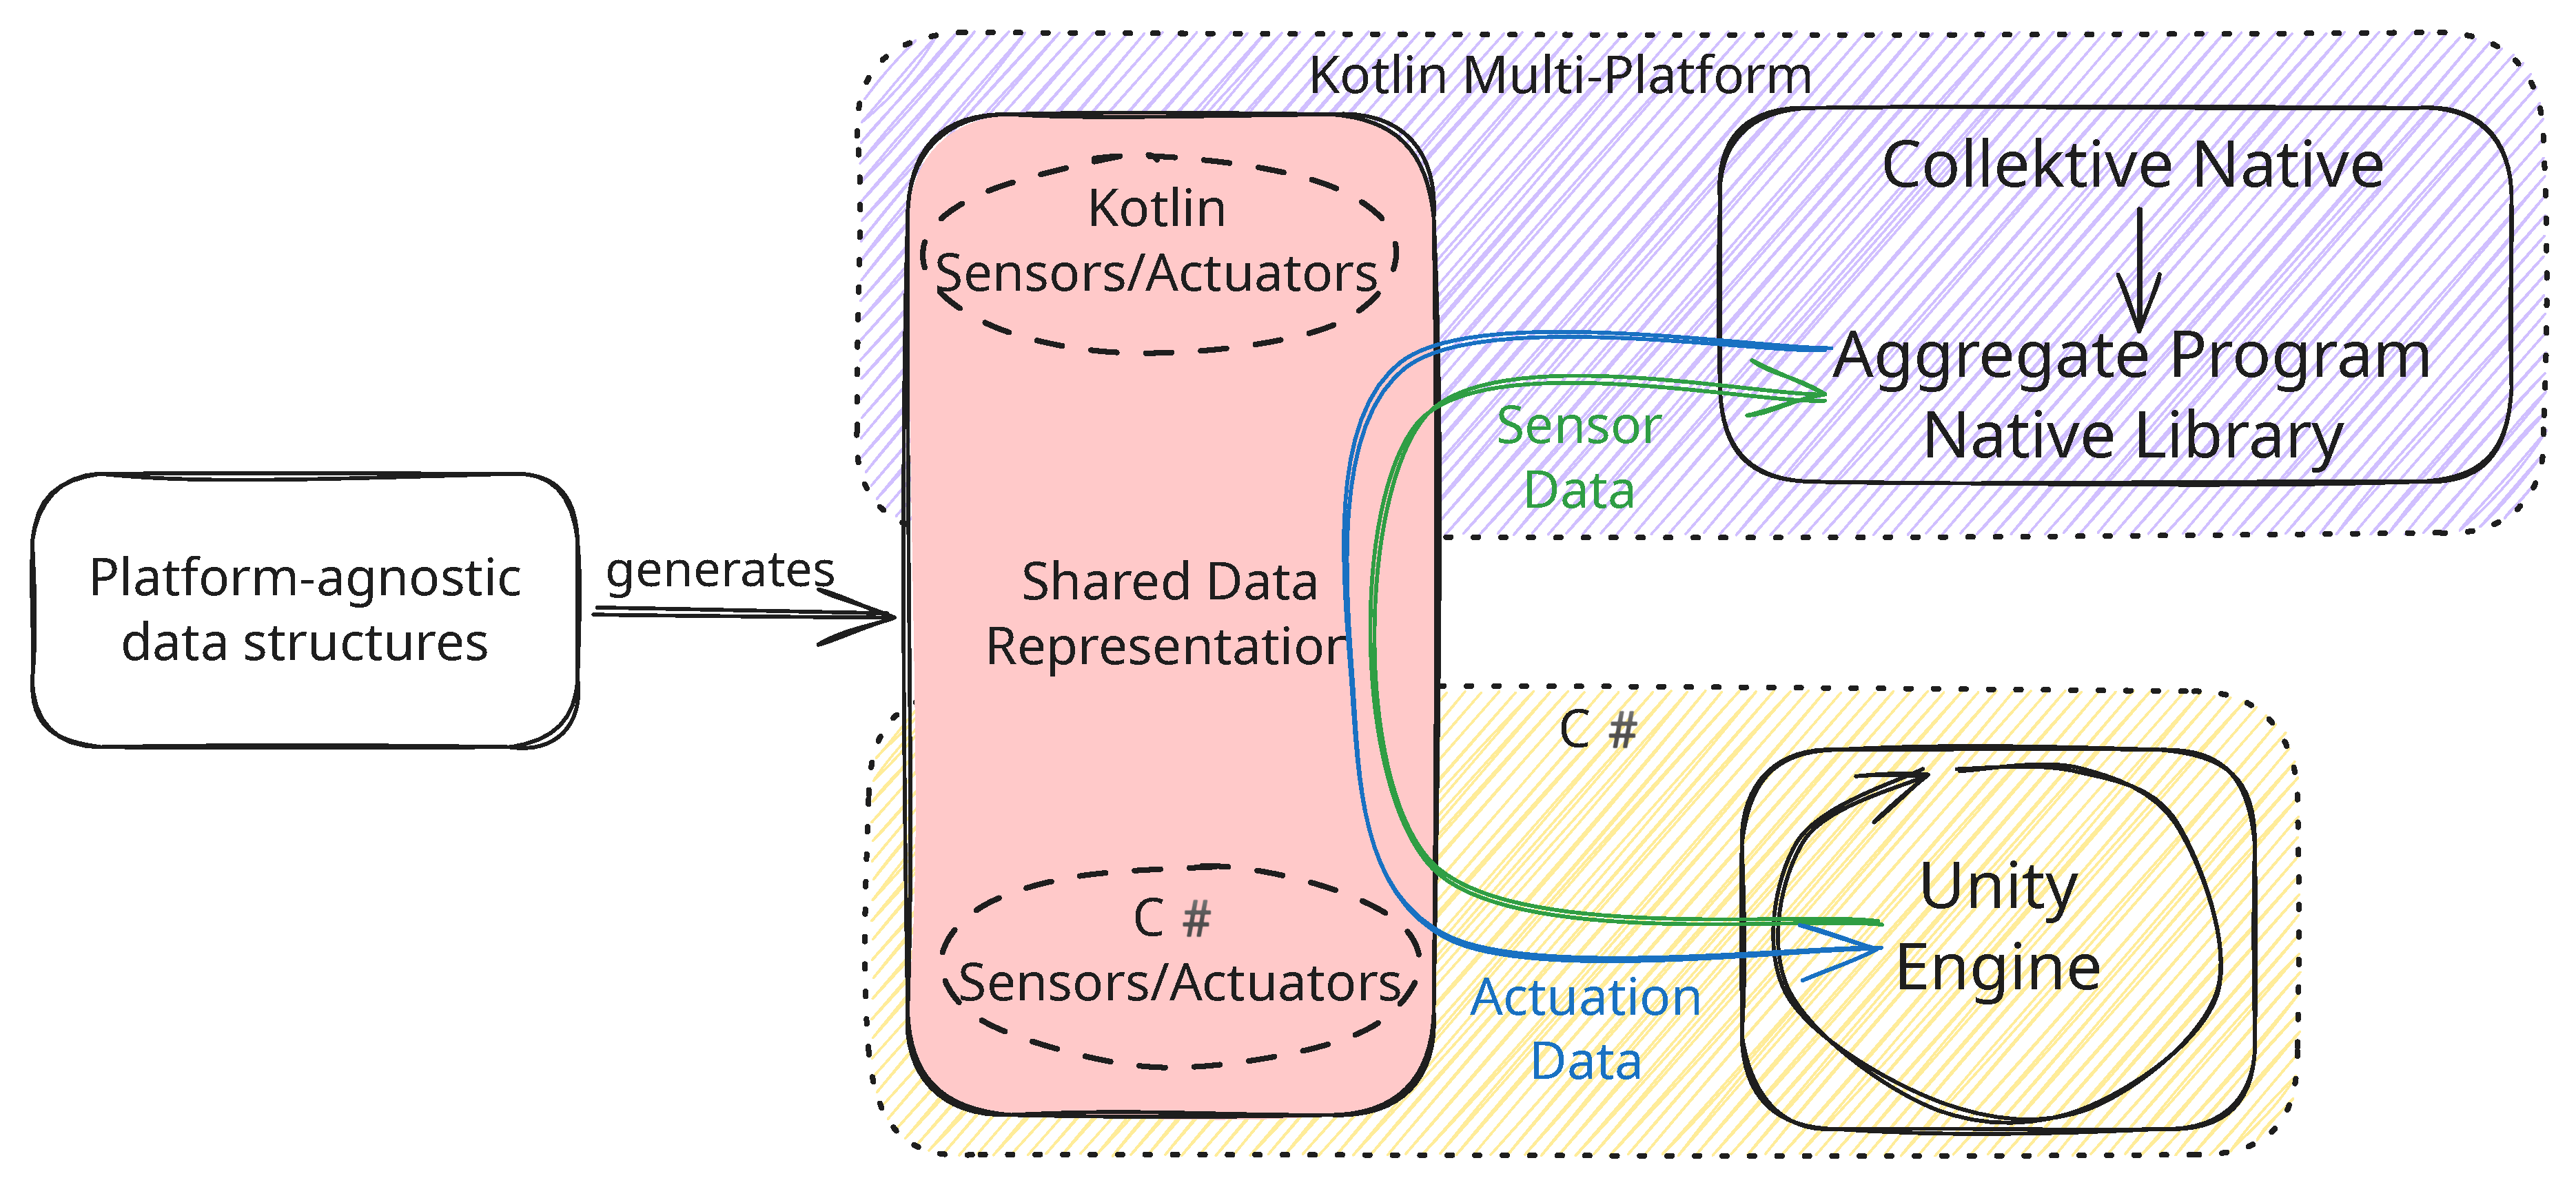
\includegraphics[width=1\textwidth]{images/architecture.pdf}
    \caption{High-level architecture of the integration between Collektive and Unity.
    %
    The Unity game engine provides Sensor Data to the Collektive aggregate program, 
    which computes Actuation Data that is sent back to the engine.
    %
    The Shared Data Representation layer allows users to define Sensors and Actuators data schema using platform-agnostic data structures,
    which are then used to automatically generate concrete data types for both platforms (i.e., Kotlin for Collektive and C\# for Unity), 
    thus enabling direct communication.
    }
    \label{fig:arch}
\end{figure}

Requirements R1 and R2 induce an architecture where data that flows between the two platforms
is structured according to a shared schema, which must be flexible enough to accommodate different use cases.
%
Since the device behavior is defined by the aggregate program,
while the environment behavior
(including physics, position in the world, and neighborhood relationships)
pertain to the game engine,
the natural division of responsibilities is to have the game engine provide sensory data to the aggregate program,
while the aggregate program computes the actuation commands back to the engine.

This architectural choice implication is that, when designing new case studies,
users must, as first step,
define the data types that represent sensors and actuators.
%
These must constitute an \emph{agnostic} layer,
expressed in a platform-agnostic format,
that must, in turn, generate bindings that enable communication between the two platforms.

Architecturally,
Unity is designed as an active component hosting a game loop,
while Collektive is designed to be executable in a purely functional style
(indeed, every aggregate program is a pure function from previous state, sensor inputs,
and neighbour messages to new state, actuation commands, and outgoing messages):
this clearly suggests that Unity should drive the execution,
and Collektive should be invoked as a library to compute the next state and actuation commands at each step of the game loop.

The architecture resulting from these considerations is illustrated in \cref{fig:arch}:
the agnostic layer generates bindings for C\# and Kotlin,
plus a shared schema for the data that flows between the two platforms.
%
Unity is the active component,
which, at each step of the game loop,
\begin{inlinelist}
    \item collects sensory data from the environment
    \item calls Collektive providing the data as input, and
    \item applies the actuation commands based on the data returned by Collektive.
\end{inlinelist}

\subsection{Integration design}\label{subsec:integration-design}

\begin{figure}
    \centering
    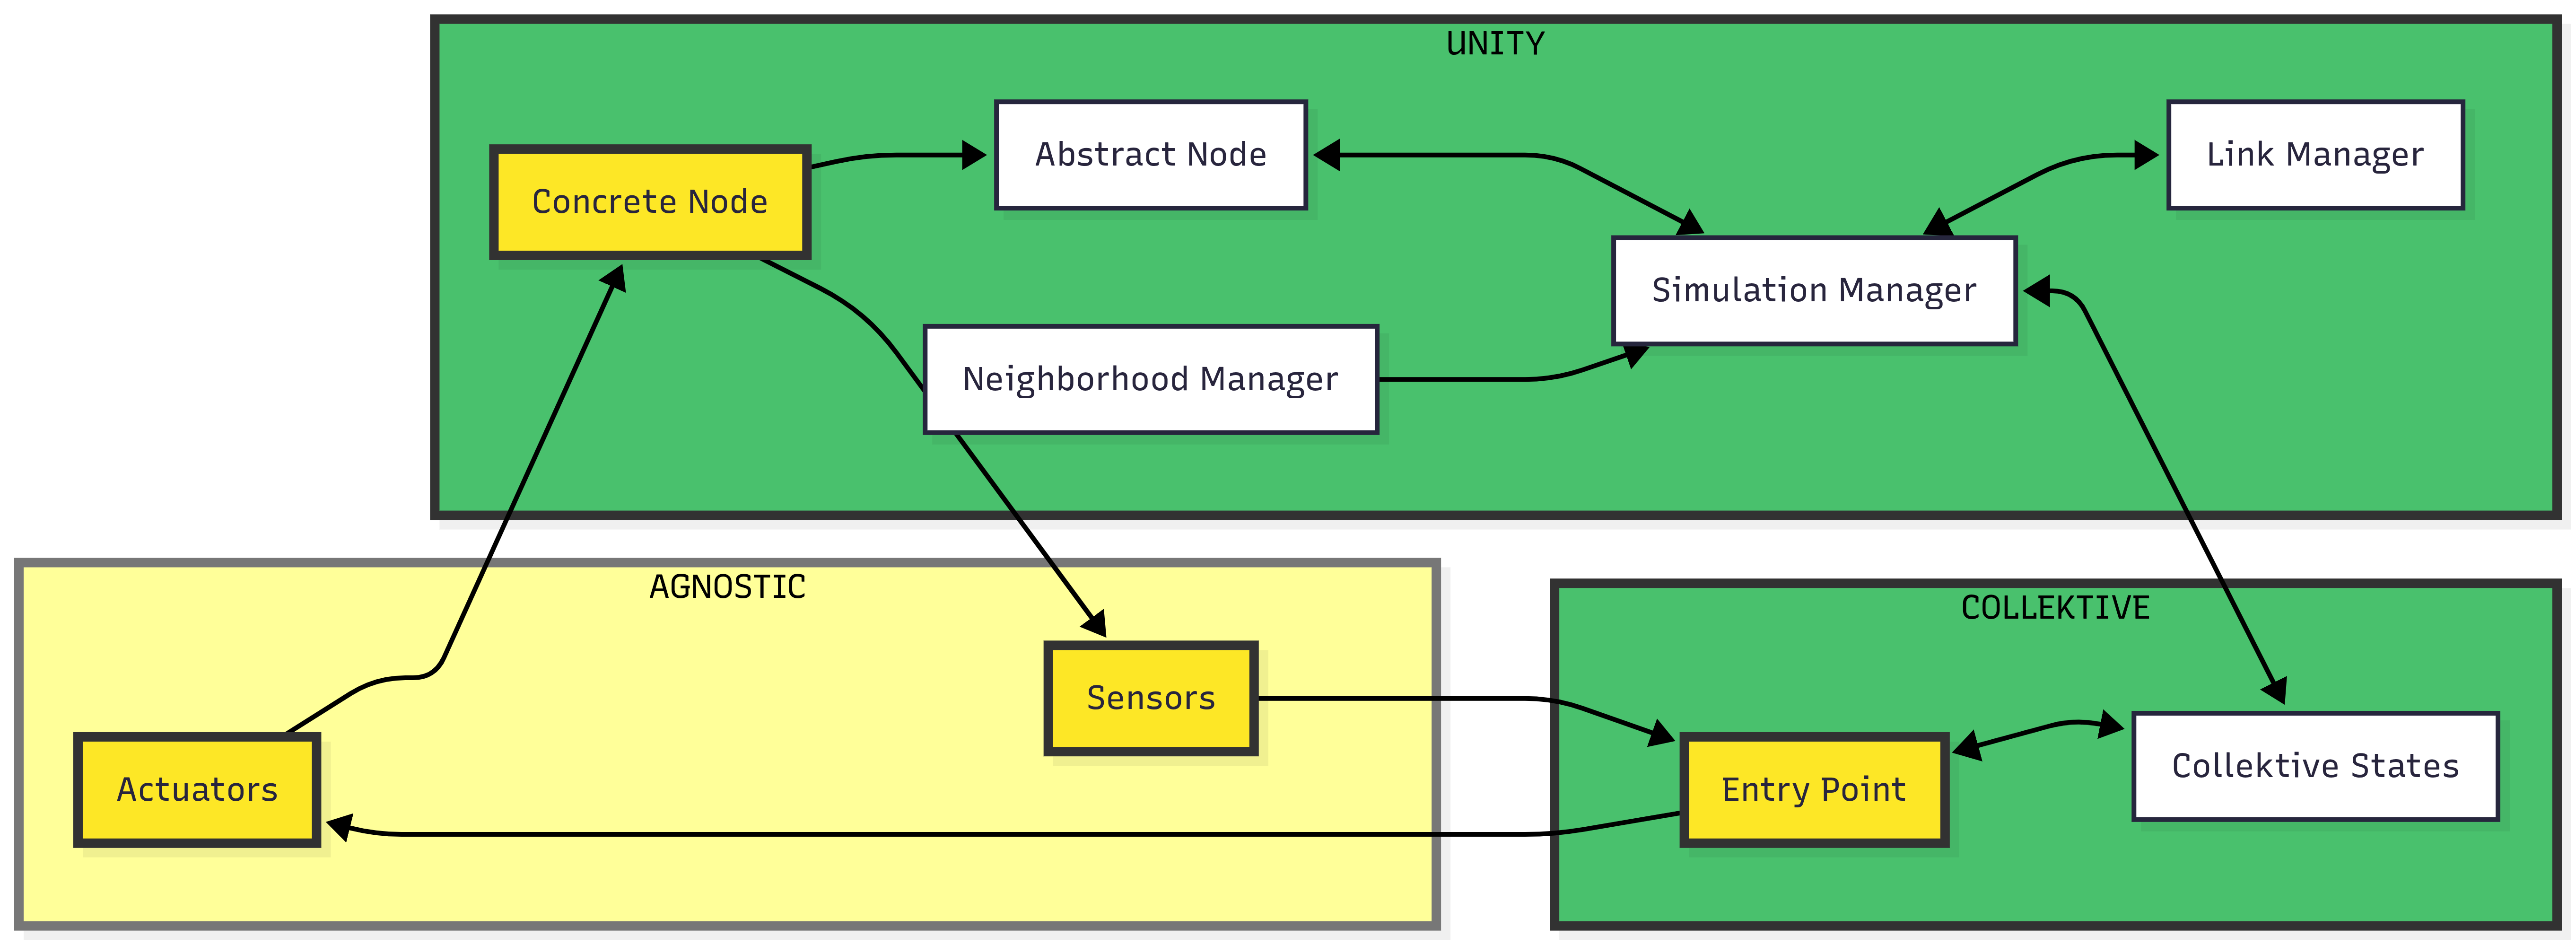
\includegraphics[width=1\textwidth]{images/design}
    \caption{
        Design of the integration layer between Collektive and Unity.
        Components highlighted in yellow must be implemented by the final user.
    }\label{fig:design}
\end{figure}

This section details the design of the integration layer that couples Unity's execution model with the Collektive runtime.
The design follows the architectural decomposition in \cref{fig:design}, separating
\begin{inlinelist}
    \item the \emph{environment layer} (Unity),
    \item the \emph{aggregate layer} (Collektive),
    and
    \item an \emph{agnostic data layer} that defines what information flows between the two.
\end{inlinelist}

\subsubsection{Agnostic data layer: sensors and actuators.}\label{sec:agnostic-data-layer}
Requirements R1 and R2 imply that the integration cannot hard-code any specific notion of sensing or actuation.
%
Instead, Collektivity exposes a thin, platform-independent contract expressed as two families of data types:
\emph{Sensors} (from Unity to Collektive) and \emph{Actuators} (from Collektive to Unity).
%
From this contract, the toolchain generates strongly typed bindings for both C\# and Kotlin, plus the marshaling code needed
to exchange values across runtimes.
%
Practically, this is realized via an \ac{IDL}-driven workflow: users describe the schema once, and code generation produces
compatible representations on both sides.
%
This choice keeps the interface stable while allowing each case study to tailor the exchanged data to its needs.

The agnostic data layer must, in the general case, be provided by the user,
as it is scenario-specific; however,
since most scenarios will likely share common sensing and actuation patterns (e.g., position, velocity, proximity, light intensity, etc.),
in the future a library of common schemas and bindings could be provided to reduce the initial overhead for new users.

%\paragraph{Native bridge and \ac{FFI}.}
%Unity scripts execute on a .NET runtime, while Collektive programs target Kotlin and, in our project, are compiled to native code.
%%
%Communication between the two can be achieved through various inter-process communication mechanisms
%(e.g., sockets, shared files, or higher-level protocols),
%or, to avoid the overhead and complexity of inter-process communication, \ac{FFI}.
%%
%Later in the paper, we'll show two implementations, based on socket and \ac{FFI}, and discuss their trade-offs.

\subsubsection{Unity-side runtime.}
Collektivity follows Unity's composition model, where behavior is defined by attaching \texttt{MonoBehaviour} components to \emph{game objects}.
The integration provides three core components.
%
\texttt{SimulationManager}
centralizes reproducibility concerns (e.g., deterministic initialization via explicit seeds) and exposes an API to create and manage links.
%
\texttt{AbstractNode} marks a game object as a Collektive device.
It defines the extension points that are scenario-specific:
how sensor data is sampled from the Unity world, and how actuator commands are applied.
%
Concrete scenarios are implemented by subclassing \texttt{AbstractNode} (e.g., \texttt{ConcreteNode} in \cref{fig:design}) and providing the
domain logic for sensing and actuation, while reusing the integration-provided communication and execution machinery.
%
\texttt{LinkManager} is a visualization-oriented singleton that maintains and renders the current network links (when enabled),
decoupling debugging/inspection concerns from simulation logic.

Aggregate programs depend on neighbor exchange, 
but the definition of \emph{who is a neighbor} is inherently situated and environment-dependent.
%
In Collektivity, 
neighborhood construction is handled by Unity, which creates and removes directed or bidirectional links through the
\texttt{SimulationManager} \ac{API}.
%
This enables multiple strategies, ranging from geometric proximity to occlusion-aware connectivity.
%
An efficient pattern leverages Unity's physics system and trigger colliders;
for instance, a connection rule component that automatically subscribes/unsubscribes links when other nodes enter/exit a proximity
volume can be implemented by annotating the implementing class with an attribute,
whose \texttt{OnTriggerEnter} and \texttt{OnTriggerExit} methods call the appropriate link-management \ac{API} to maintain the neighborhood structure.
%
%\begin{verbatim}
%[RequireComponent(typeof(Collider))]
%public class ProximityNeighborhoodBehaviour : MonoBehaviour {
%  private Collider _collider;
%  private Node _node;
%
%  private void Start() {
%    _collider = GetComponent<Collider>();
%    _node = GetComponentInParent<Node>();
%  }
%
%  private void OnTriggerEnter(Collider other) {
%    var otherNode = other.GetComponent<Node>();
%    if (otherNode != null) {
%      SimulationManager.Instance.Subscribe(_node, otherNode);
%    }
%  }
%
%  private void OnTriggerExit(Collider other) {
%    var otherNode = other.GetComponent<Node>();
%    if (otherNode != null) {
%      SimulationManager.Instance.Unsubscribe(_node, otherNode);
%    }
%  }
%}
%\end{verbatim}
%
By delegating neighborhood dynamics to Unity, the integration can directly reuse engine-level facilities (collisions, triggers, layers, and spatial
partitioning), while keeping the Collektive runtime agnostic of the specific spatial model.

At each simulation tick, Unity performs the following steps for each node:
\begin{inlinelist}
    \item sample sensors from the world state,
    \item invokes the Collektive adapter,
    which evaluates the aggregate program provided the most recent messages from current neighbors and the last device state,
    returning actuation commands,
    and
    \item apply actuators to Unity objects.
\end{inlinelist}
%
This design preserves the functional structure of aggregate rounds while fitting Unity's imperative update loop, and provides a single place
(\texttt{SimulationManager}) to enforce scheduling policies (e.g., fixed-rate stepping) and to coordinate message delivery.

Collektivity provides the implementation for the \texttt{SimulationManager}, the \texttt{AbstractNode}, and the \texttt{LinkManager},
plus the code-generation workflow for Sensors/Actuators.
%
Scenario developers provide:
\begin{inlinelist}
    \item the sensor/actuator schema,
    \item concrete node components that interpret the schema and implement sensing/actuation, and
    \item neighborhood rules implemented as Unity components that call the link-management \ac{API}.
\end{inlinelist}

\subsubsection{Collective-side \ac{API}}\label{subsec:collective-api}

On the Collektive side, Collektivity exposes a minimal \ac{API} that wraps the execution engine and
presents it as a stateful service to the Unity runtime.
This \ac{API} has two goals:
\begin{inlinelist}
    \item provide Unity with a stable entry point to advance the aggregate computation for each device, and
    \item internalize all program-dependent artifacts (in particular, neighbor message contents and device state),
    so that the Unity integration remains independent of the specific aggregate program.
\end{inlinelist}

In aggregate computing, the shape of the messages exchanged among neighbors is not an application-level design choice:
it is induced by the program structure and by the compilation strategy of the underlying calculus~\cite{DBLP:journals/tocl/AudritoVDPB19}.
%
Consequently, modeling messages as part of the Unity-side schema would undermine R1:
every change in the aggregate program could require regenerating schemas and bindings and revising Unity-side code,
which is not sustainable for iterative development and experimentation.
%
For this reason, Collektivity treats neighbor messaging as an internal concern of the Collektive runtime, not as part of the
Sensors/Actuators contract.
%
Thus, the collective-side \ac{API} maintains, for each simulated device:
\begin{inlinelist}
    \item the latest \emph{device state} produced by the aggregate program (used to support stateful constructs across rounds),
    \item the most recent \emph{inbound messages} received from current neighbors, and
    \item the \emph{outbound messages} generated in the last round, which will be delivered to neighbors according to the topology provided by Unity.
\end{inlinelist}
In addition, it stores the association between Unity node identifiers and Collektive engine instances,
so that Unity can refer to devices through stable handles.

At each simulation tick, Unity invokes the collective-side \ac{API} to advance each device by one round.
For a given device, the \ac{API} evaluates the aggregate program against
\begin{inlinelist}
    \item the stored device state,
    \item the current sensor snapshot provided by Unity,
    and
    \item the inbound messages buffered from neighbors.
\end{inlinelist}
%
The evaluation produces a new device state, a set of outbound messages, and the actuator commands.
%
Unity then applies the returned actuators to update the game objects, and uses its current link graph to determine how outbound messages
are routed to neighbor buffers before the next tick.
%
This division of responsibilities matches the architecture in \cref{fig:design}:
Unity owns the environment and the topology,
while Collektive owns the distributed computation semantics.

\subsection{Implementation strategy}\label{subsec:implementation}

In this section,
we describe the practical construction of Collektivity,
discussing the technological choices that realize the design outlined in \Cref{subsec:integration-design}.
%
The implementation of Collektivity is publicly available\footnote{\url{https://github.com/pslab-unibo/collektivity}}
and archived for future reference~\cite{collektivity-zenodo},
and has the form of a repository template.
%
The purpose of the template is to provide a starting point for researchers and practitioners interested in
integrating experimenting with aggregate programs in Unity.

\begin{table*}[t]
    \centering
    \caption{Performance comparison between the native (\ac{FFI}) and socket-based backends.
    Times are in nanoseconds (ns), lower is better.
    Speedup is reported as Socket/Native (higher is worse for sockets).}
    \label{tab:backend-frontend-benchmark}
    \setlength{\tabcolsep}{6pt}
    \renewcommand{\arraystretch}{1.15}
    \begin{tabular}{l | r | r | r | r | r | r}
        \hline
        \textbf{Metric} & \multicolumn{3}{c |}{\textbf{Overhead Collektive-side}} & \multicolumn{3}{c}{\textbf{End-to-end (ns)}} \\
        \cline{2-4}\cline{5-7}
        & \textbf{FFI} & \textbf{Socket} & \textbf{Speedup} & \textbf{Native} & \textbf{Socket} & \textbf{Speedup} \\
        \hline
        count  & 970 & 969 & -- & 969 & 968 & -- \\
        median & 13830 & 137857 & 11.20$\times$ & 550600 & 200001950 & 363.32$\times$ \\
        mean   & 13175 & 170269 & 13.86$\times$ & 484754 & 199963813 & 456.26$\times$ \\
        p95    & 16597 & 348890 & 28.02$\times$ & 612140 & 200560775 & 719.35$\times$ \\
        p99    & 36306 & 456583 & 41.25$\times$ & 850520 & 202753798 & 747.95$\times$ \\
        std    & 4843  & 265368 & -- & 141814 & 3265095 & -- \\
        \hline
    \end{tabular}
\end{table*}

As first step to head into implementation,
we built an experimental prototype with 12 nodes to compare the performance of two communication strategies
through a simple benchmark that simulates the core communication pattern of Collektive programs:
\begin{inlinelist}
    \item a socket-based backend, where Unity and Collektive run as separate processes and exchange data through TCP sockets, and
    \item a native backend, where Collektive is compiled to a shared library and directly invoked by Unity through \ac{FFI}.
\end{inlinelist}
%
We expected better performance for the latter,
but the former has the advantage of being more flexible,
as any Collektive target could be used,
instead of limiting the support to the native compilation targets.
%
The benchmark is publicly available\footnote{
    \scriptsize
    \url{https://github.com/pslab-unibo/experiment-2026-coordination-collektive-unity-benchmark}
} and archived for future reference~\cite{benchmark-zenodo}.
%
\Cref{tab:backend-frontend-benchmark} summarizes the results.
%
The performance difference is stark: the socket-based backend is, on average,
over 450x slower than the native backend,
with a worst-case slowdown of over 700x.
%
Provided the relevance of R3, we adopted the native compilation strategy for the integration,
and we designed the agnostic data layer to support it.

\subsubsection{Data Model}\label{sec:data-model-and-serialization}

Collektive and Unity use different type systems and memory layouts.
%
As discussed in \Cref{sec:agnostic-data-layer},
a shared data model representation,
expressed in a platform-agnostic format, 
is essential to enable communication between the two platforms while maintaining flexibility and extensibility.
%
%In such way,
%users can define the data schema once,
%and the toolchain generates the bindings to its use in both platforms (i.e., C\# and Kotlin).
%
%For data representation,
%one could consider using widely adopted serialization formats---%
%for instance, JSON or XML.
%%
%In order make use of such information representation,
%both Collektive and Unity should additionally require to
%\begin{inlinelist}
%    \item define a common schema for the data to be exchanged, which is dependent on the specific requirements of the application, and
%    \item provide parsers and serializers implementations for each information schema.
%\end{inlinelist}
%%
%Such approach, howerver,
%lacks efficiency, because the modification of the data schema must be reflected on both C\# and Kotlin code,
%therefore not satisfying requirement R1.
%%
%Moreover,
%type-safety is not guaranteed,
%as the data is represented as unstructured text.
%
%There exist other approaches to data representation and serialization that can better fit
%the requirements of our integration.
%
\emph{Protocol Buffers}\footnote{\url{https://protobuf.dev/}} (\texttt{protobuf}) is a language-neutral,
platform-neutral mechanism for serializing structured data.
%
Protocol Buffers defines data models using a declarative syntax (\texttt{.proto} files)
that describes their structure in an implementation-agnostic way.
%
From a single \texttt{.proto} definition,
the \texttt{protoc} compiler can generate serialization source code for multiple languages automatically,
including C\#, Kotlin, Java, and many others.
%
Protocol Buffers data structures are defined as \texttt{messages},
which are composed of fields with a type and a unique identifier (tag).
%
In our use case,
we always have exactly two messages: one for \texttt{Sensors} and one for \texttt{Actuators}
(indeed, the \texttt{message}s of protocol buffers are \emph{not} the messages that aggregate programs exchange,
rather, they describe the data that is exchanged with Unity).
%
Each field can be a primitive type (e.g., integer, string, boolean)
or a user-defined message type,
allowing for nested and complex data structures.
%
The tag is used to identify fields in the binary format, 
enabling efficient serialization and deserialization.
%
This makes Protocol Buffers fit for bridging complex data model representation for Kotlin and C\# runtimes.
%
In Collektivity, 
users define \texttt{Sensors} and \texttt{Actuators} data schema using Protocol Buffers,
the latter will then generate the necessary bindings for both platforms.
%
A minimal example of a Protocol Buffers schema for Sensors and Actuators is shown in \Cref{lst:proto-schema}.
%
Depending on the specific requirements of the application,
users can define more complex data structures.
%including nested messages, repeated fields, and optional fields.

\begin{lstlisting}[
    basicstyle=\ttfamily,
    linewidth=\textwidth,
    caption={
        Example of Protocol Buffers schema for Sensors and Actuators.
        %
        \texttt{sourceIntensity} is a \texttt{double} field used by the aggregate program to determine the direction of movement towards the destination.
        %
        \texttt{Vector3} maps a Unity 3D vector, which in this example represents the current position of the device and the target position computed by the aggregate program.
        %
        \texttt{repeated Vector3} represents a list of 3D vectors, which in this example represent obstacles positions.
        %
        The integer tags (e.g., \texttt{= 1}) are used to identify fields in the binary format.
    },
    label={lst:proto-schema},
]
message Actuators {
  Vector3 targetPosition = 1;
}
message Sensors {
  double sourceIntensity = 1;
  Vector3 currentPosition = 2;
  repeated Vector3 obstacles = 3;
}
\end{lstlisting}

%\subsection{Information Exchange between Unity and Collektive}
%
%To facilitate the flow of information between Unity and Collektive,
%a communication mechanism is required for transmitting sensor data and actuator information.
%%
%Following the requirement for high-performance interoperability (R3),
%the wo viable options for communication identified are
%\ac{FFI} and socket-based communication.
%
%\ac{FFI} allows direct interaction between different programming languages
%by enabling one language to call functions or use data types defined in another language.
%%
%In this context,
%it allows Unity (C\#) to directly invoke functions from Collektive (Kotlin).
%%
%This approach facilitates efficient data exchange without the overhead of inter-process communication.
%
%On the other hand,
%socket-based communication involves establishing a network connection between Unity and Collektive,
%allowing them to send and receive messages over a network protocol.
%%
%This approach is flexible,
%since it is based on an external and independent component (i.e. a server) which offers a standard interface between the two languages and it is stand-alone---%
%i.e., it can be developed and tested independently from the rest of the system.
%%
%To determine the most performant option that satisfies R3,
%we conducted a benchmark comparing the two methods aforementioned,
%which is detailed in \Cref{sec:case-study}.
%
%Based on the results of this benchmark,
%we chose to implement \ac{FFI} in Collektivity,
%as it provided significantly lower latency and better performance for the integration.

\subsubsection{\ac{FFI} interaction and Engine API}

Collektivity extends the Collektive runtime to support execution within the Unity environment,
to do so, it provides an \texttt{Engine} (\Cref{lst:engine-api})
that defines the contract between the aggregate program and the Unity environment---%
i.e., the operations that Unity can invoke on the Collektive runtime to execute the aggregate program and retrieve the resulting state and actuation commands.
%
\texttt{Engine} is the Collektive interface that Unity invokes to execute the aggregate computation at each simulation tick,
i.e. each update cycle in the Unity execution loop triggers the invocation 
of the \texttt{step()} function in the \texttt{Engine}.
%
This function is invoked by Unity via \ac{FFI} for each simulation node, 
which identifier is specified during invocation along with \texttt{Sensors} data structure.
%
The result returned by Collektive is an \texttt{Actuators} data structure,
which is then used by Unity to update the simulation environment accordingly.
%
\texttt{Sensors} and \texttt{Actuators} are defined in the agnostic data layer,
and their schema is defined by the user (c.f., \Cref{sec:data-model-and-serialization}).

\lstinputlisting[
    % float,
    basicstyle=\scriptsize\ttfamily,
    linewidth=\textwidth,
    language=Kotlin,
    caption={Engine API definition for Collektive library.},
    label={lst:engine-api},
]{listings/Engine.kt}

Along with the \texttt{step()} function,
\texttt{Engine} also defines methods for
\begin{inlinelist}
    \item register a node for being neighbor of another node (i.e., using \texttt{subscribe()}), 
    \item unregister a node from being neighbor of another node (i.e., using \texttt{unsubscribe()}),
    \item add a node to the simulation (i.e., using \texttt{addNode()}), and
    \item remove a node from the simulation (i.e., using \texttt{removeNode()}).  
\end{inlinelist}
%
This infrastructure is then compiled using Collektive-native,
and it is directly invoked by Unity via \ac{FFI}.

\section{Exemplars}\label{sec:case-study}

In this section,
we show a simple and a richer exemplar that we include with Collektivity
to demonstrate its capabilities and to provide a starting point for users interested in experimenting with aggregate programming in Unity.
%
In both exemplars,
we deploy devices that must navigate towards a source of interest while avoiding obstacles,
which is a common pattern in \acp{CAS} and is relevant for a wide range of applications (e.g., search and rescue).
%
They do so through a gradient ascent strategy, with no cooperative logic is implemented for obstacle avoidance.
%
All nodes execute synchronous rounds at a fixed frequency of $20Hz$,
in which they perceive the local ``intensity'' of the source of interest (based on the distance)
and detect obstacles in their vicinity.
%
Vicinities and communication between nodes are established through a distance-based neighborhood model:
two nodes are considered neighbors if their separation is within 10 units,
which defines the connectivity graph for the aggregate computation.
%
They exchange this information with their neighbors to compute their next movement direction,
computing a vector that points to the direction of higher source intensity and away from nearby obstacles
(including other devices).
%
Gradient computations are performed through the standard library in Collektive,
which provides implementations for all the building blocks in~\cite{DBLP:journals/tomacs/ViroliABDP18}.

\subsection{Simple 3D space}

\begin{figure}
    \centering
    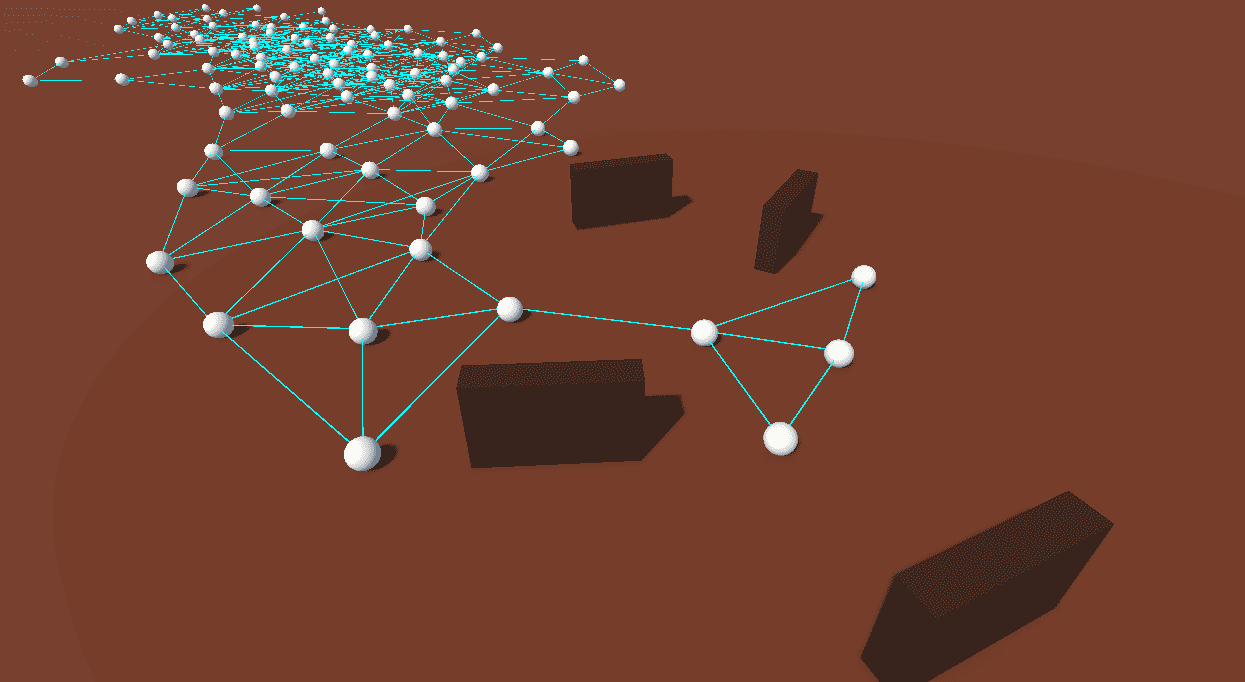
\includegraphics[width=.49\textwidth]{images/simple-shots/better_1}
    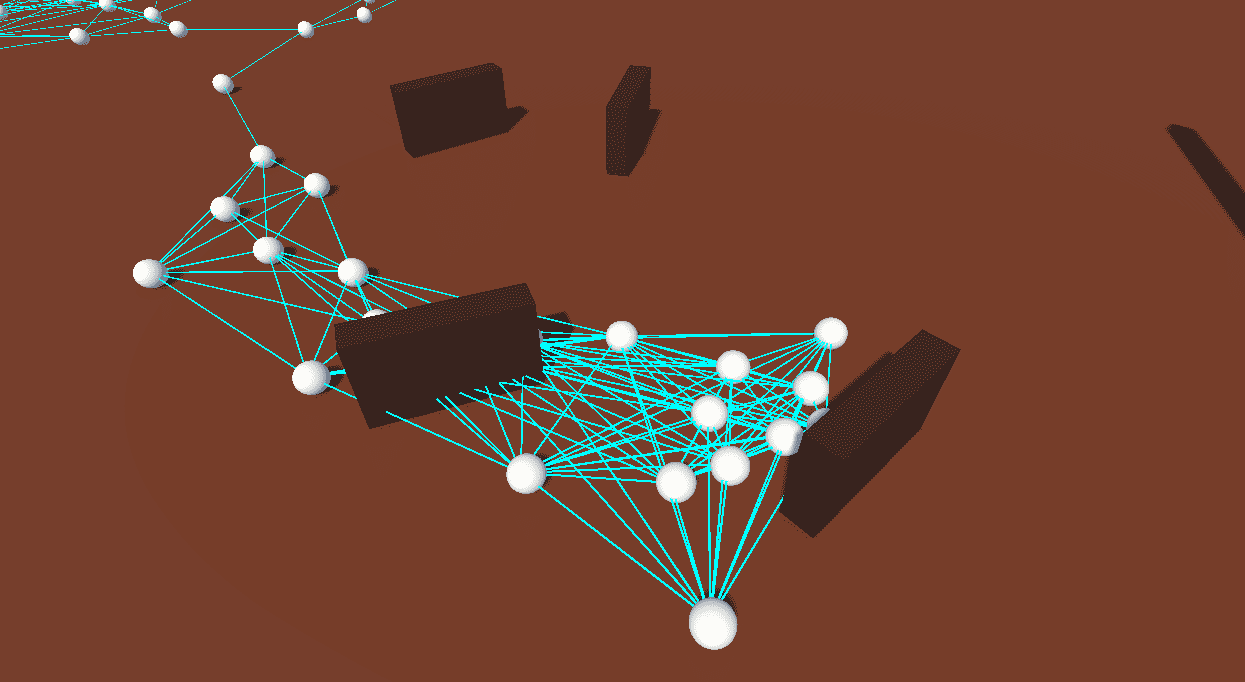
\includegraphics[width=.49\textwidth]{images/simple-shots/better_2}
    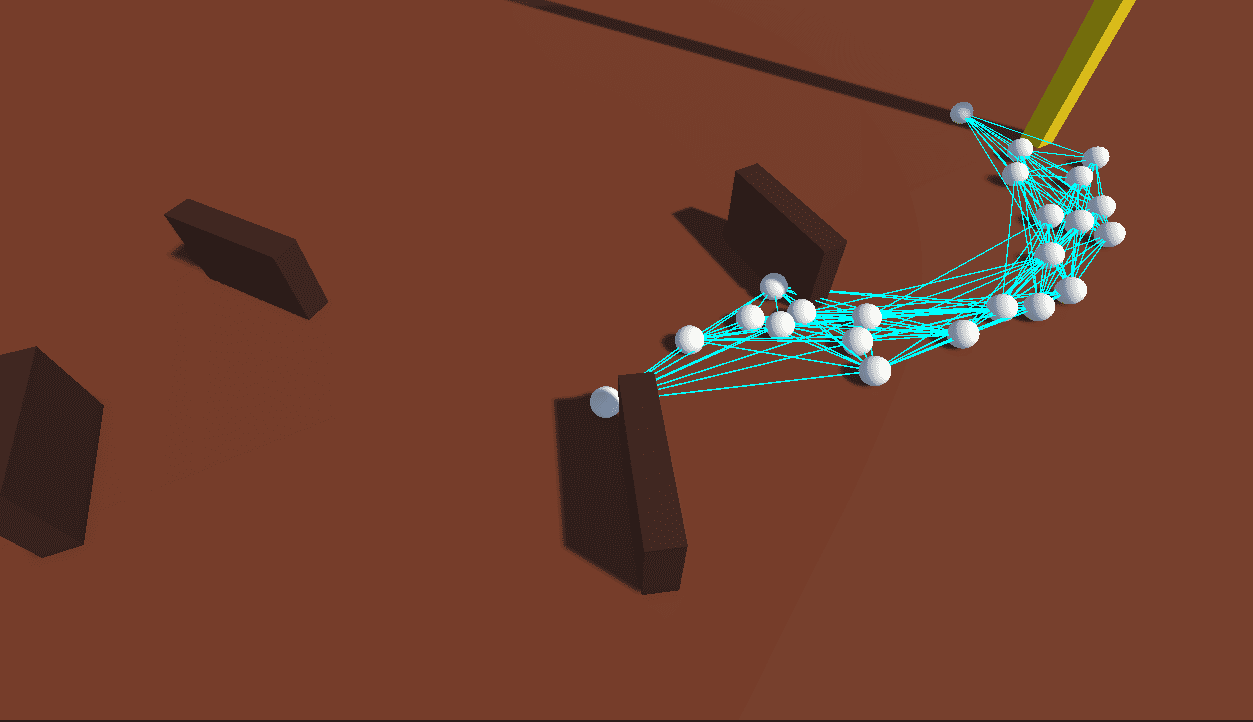
\includegraphics[width=.49\textwidth]{images/simple-shots/better_3}
    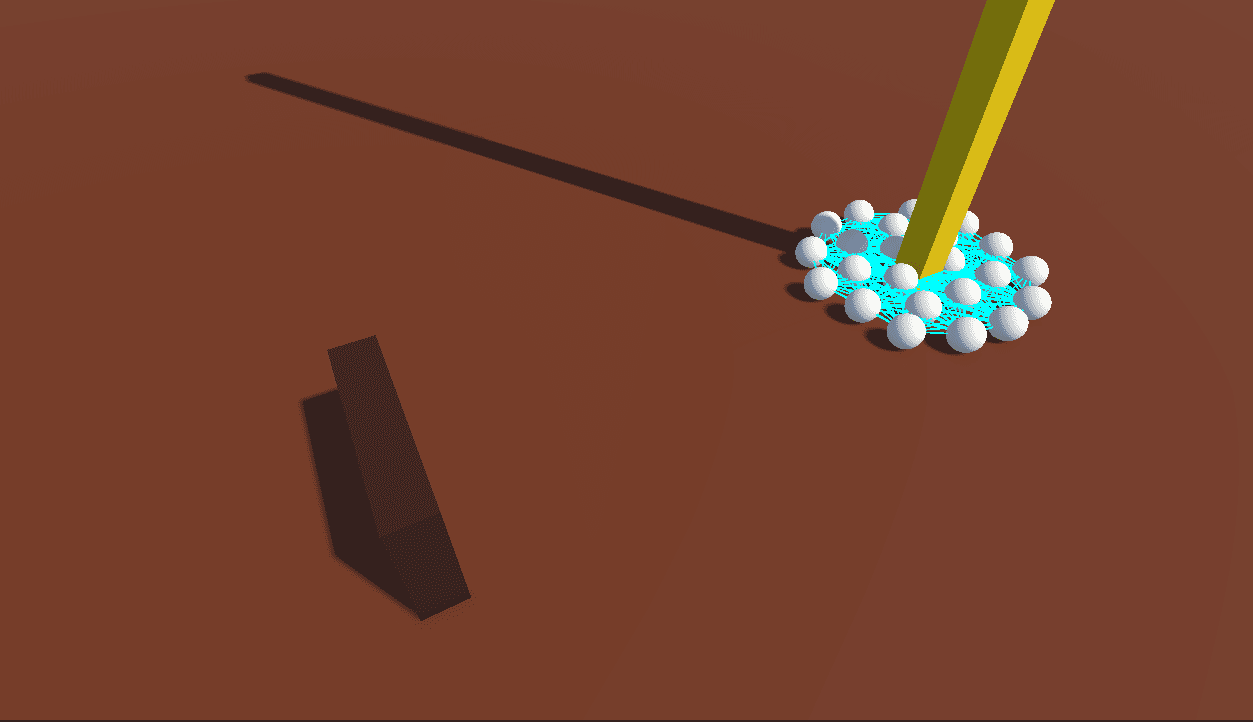
\includegraphics[width=.49\textwidth]{images/simple-shots/better_4}
    \caption{Snapshots of the simple 3D space scenario with 100 nodes.}\label{fig:simple}
\end{figure}

Here, we consider a simple arena with
four parallelepipedic obstacles that physically obstruct the movement towards the source.
The environment contains  of $1 \times 3 \times 5$ units.
%
Devices are represented by spheres that can move in the 3D space,
and the arena is a flat plane with a source of interest located at a fixed position.
%
We tested the scenario with different numbers of nodes.
%
Laptops with integrated graphics could achieve reasonable real-time performance with up to 50 nodes,
while we easily scaled to 100 nodes on a desktop with a dedicated GPU (nVidia GTX 4070).
%
Snapshots in \Cref{fig:simple} show the evolution of the system with 100 nodes.

\subsection{Richer environment}

%\danilo{fate una selezione di quattro snapshot fra quelli che ho messo in images/complex e fate un'immagine migliore}

\begin{figure}
    \centering
%    \includegraphics[width=.49\textwidth]{images/oasis/01}
    \includegraphics[width=.49\textwidth]{images/oasis/02}
    \includegraphics[width=.49\textwidth]{images/oasis/03}
%    \includegraphics[width=.49\textwidth]{images/oasis/04}
    \includegraphics[width=.49\textwidth]{images/oasis/05}
    \includegraphics[width=.49\textwidth]{images/oasis/06}
    \caption{Snapshots of the Oasis scenario with 100 nodes.}\
    \label{fig:oasis}
\end{figure}


To showcase the potential of this integration,
we ran the same experiment in one of Unity's built-in environments (i.e., ``Oasis'').
%
In this scenario, obstacles are represented by trees, bushesh, and rocks,
and the source of interest is located inside a tent located on the opposite side of the arena
with respect to the initial placement of the nodes.
%
Snapshots in \Cref{fig:oasis} show the evolution of the system with 100 nodes.
%
This scenario had to be executed on the better equipped desktop to retain real-time performance,
as the increased complexity of the environment
(e.g., more complex geometry, more detailed rendering, and more complex physics interactions)
significantly impacted the performance of the simulation.

\section{Conclusion and Future Work}\label{sec:conclusion}

In this work we presented Collektivity,
a toolchain for the execution of aggregate programs written 
in Collektive on top of the Unity game engine.
%
This integration enables to leverage Unity's physics capabilities 
to create realistic and general-purpose simulations for testing and validating \acp{CAS}.

To achieve this integration,
we designed an architecture to unify the execution model of Unity with the functional nature of aggregate programs,
we extended the Unity engine to support the direct invocation of Collektive computations through \ac{FFI},
while using a shared platform-agnostic data model using Protocol Buffer.
%
To guide the design and implementation of Collektivity, 
we conducted a benchmark to compare the performance of \ac{FFI} and socket-based communication strategies, 
which informed our decision to adopt \ac{FFI} for the integration.
%
Finally, 
we show two examples of unity applications that demonstrates the opportunities of running Collektive on top of Unity,
both of them provided as a starting point for users interested in experimenting with aggregate programming in Unity.

As future work, 
we plan to provide additional example scenarios that showcase more complex aggregate computations,
also including larger populations (e.g., 1{,}000 and 10{,}000 nodes) to demonstrate the scalability of the integration.
%
This will offer users a broader reference set of examples for building their own simulations, 
thereby lowering the entry barrier for experimenting with aggregate programming in Unity.
%
We also plan to compare the current implementation with an \ac{ECS}-based one,
which is a design pattern widely adopted in game development and recently supported by Unity through its \ac{DOTS} framework\footnote{\url{https://unity.com/dots}}.

As discussed in \Cref{subsec:requirements},
the main technical and design challenges encountered in the integration are expected to recur,
at least in part, in other game engines.
%
To assess this hypothesis,
we plan to integrate Collektive with another game engine, such as Unreal Engine or Godot.
%
This would help evaluate the generality of the proposed design and identify which aspects transfer across engines
and which require engine-specific solutions.

\bibliographystyle{splncs04}
\bibliography{paper-2026-coordination-unity-collektive}

%\begin{appendix}
%\section{Companion Artefact Description}
%\subsection{Badge Claims}
%
%\subsubsection{Available}
%The complete source code, and instructions to reproduce the simulations
%presented in the paper are publicly accessible at \url{https://github.com/pslab-unibo/collektivity}
%and archived at \url{https://zenodo.org/doi/10.5281/zenodo.18761590}.
%
%\subsubsection{Reusable}
%The artefact is provided as a repository template,
%providing instructions on how to reproduce the experiments and
%how to extend it to build and simulate custom Collektive aggregate computations in Unity,
%enabling researchers and practitioners to adapt it to their own experiments.
%The documentation, provided in the artefact's README,
%includes also the requirements for running the simulations,
%and a brief description of the architecture and design of the integration.
%
%\subsubsection{Functional outcomes}
%The artefact enables the execution of aggregate programs written in Collektive within the Unity game engine,
%demonstrating the support for realistic environment simulations of collective adaptive systems.
%%
%The provided examples demonstrate navigation and obstacle avoidance in both simple and rich Unity scenes.
%
%\subsubsection{Reusability claims}
%
%Collektivity is designed as a repository template,
%allowing users to instantiate new projects with minimal additional configuration.
%%
%The platform-agnostic data layer and code generation workflow facilitates the project capability to adapt to diverse scenarios.
%%
%Researchers can extend the artefact by defining new \texttt{SensorData} and \texttt{ActuatorData} schemas,
%and proceed to implement custom aggregate programs upon these data structures,
%while leveraging Unity's features for environment modeling and visualization.
%%
%The documentation guides users through these customization steps.
%
%\subsection{Quick Start}
%
%\subsubsection{Kick-the-Tires Instructions}
%
%The execution of the experiments requires \textbf{Linux} or \textbf{macOS} operating systems,
%for which the provided instructions are tested and guaranteed to work.
%
%To run the provided simulations, follow these steps:
%
%\begin{enumerate}
%    \item \textbf{Install Java 21}:
%    Verify the installation with: \texttt{java -version}.
%    It should print a version string containing \texttt{21}.
%    \item \textbf{Install Unity Hub}:
%    \begin{itemize}
%        \item Follow the official instructions from \url{https://unity.com/download}.
%        \item Launch Unity Hub
%        \item Create a Unity account and log in.
%    \end{itemize}
%    \item \textbf{Install Unity Editor 6000.3.8f1}:
%    \begin{itemize}
%        \item Open Unity Hub.
%        \item Go to the \texttt{Installs} tab.
%        \item Click \texttt{Install Editor}.
%        \item Select version \texttt{6000.3.8f1} from the list and install.
%    \end{itemize}
%
%    \item \textbf{Install Node.js and npm}:
%    \begin{itemize}
%        \item Download and install Node.js (which includes npm) from \url{https://nodejs.org/}.
%        \item Recommended versions: Node.js v25.6.1, npm 11.9.0 (other recent versions should work).
%        \item Verify installation with: \texttt{node -v} and \texttt{npm -v}
%    \end{itemize}
%    \item \textbf{Import the Project}:
%    \begin{itemize}
%        \item Clone the project repository
%        \begin{itemize}
%            \item \texttt{git clone \url{git@github.com:pslab-unibo/collektivity.git}}
%        \end{itemize}
%        \item In Unity Hub, go to the \texttt{Projects} tab.
%        \item Click \texttt{Add} and \texttt{Add Project from Disk}.
%        \item Browse to the \texttt{Sandbox.Collektive.Unity} folder in the artefact.
%        \item Select it and confirm.
%        \item Install the recommended Unity packages if prompted (the installation may take a few minutes).
%    \end{itemize}
%
%    \item \textbf{Open the Project in Unity Editor}:
%    \begin{itemize}
%        \item Double-click the project entry in Unity Hub.
%        \item Read and accept the Unity Editor Software terms and conditions if prompted.
%        \item Unity Editor will launch and load the project (note that it is not executable yet)
%        \item In the top bar, click \texttt{Tools}, then run both \texttt{Proto > Generate} and \texttt{Native > Rebuild backend}.
%        \begin{itemize}
%            \item if the environment does not respond after two minutes, send a kill signal to the Unity Editor process and restart it, then repeat this step.
%        \end{itemize}
%        \item In the \texttt{Project} tab, navigate to \texttt{Assets/Scenes} and double-click \texttt{Robots and Obstacles.unity} to open the scene.
%        \item Press the \texttt{Start} button at the top center of the Unity Editor to launch the simulation.
%    \end{itemize}
%
%\end{enumerate}
%
%If the steps succeed without incurring in errors,
%you should be able to run the provided simulations.
%
%
%\paragraph{Fast Troubleshooting.}
%On macOS, the simulation may fail to start if Xcode has not been initialized yet.
%This happens because the native backend relies on Apple's developer toolchain
%(e.g., \texttt{xcrun}) that becomes available only after Xcode completes its first-time setup:
%\begin{itemize}
%    \item If Xcode is already installed, open it at least once and accept the license agreement.
%          This step finalizes the installation of the required Command Line Tools;
%    \item If Xcode is not installed, install it from the App Store, launch it once,
%          and accept the license agreement when prompted.
%\end{itemize}
%
%After this initialization step, rerun the build (\texttt{Proto > Generate} and \texttt{Native > Rebuild backend});
%the simulation should start normally.
%
%If you encounter a Win32Exception error related to \emph{npx} or \emph{protoc},
%ensure Node.js and npm are installed.
%%
%The Proto > Generate step uses \texttt{npx protoc} to invoke the Protocol Buffers compiler.
%
%\subsubsection{Project Structure}
%The project is structured as follows:
%
%\begin{itemize}
%    \item \texttt{collektivity/} -- Main project root
%    \item \texttt{collektive-backend/} -- Backend library for Collektive computation
%    \begin{itemize}
%        \item {\scriptsize\texttt{lib/src/commonMain/kotlin/it/unibo/collektive/unity/examples}} -- Collektive entrypoint for the aggregate program
%        \item {\scriptsize\texttt{lib/src/commonMain/proto/user-defined-schema.proto}} -- Protobuf definition for user defined data schema
%    \end{itemize}
%    \item \texttt{Collektive.Unity/} -- Unity engine integration to invoke Collektive computation
%    \begin{itemize}
%        \item \texttt{Runtime/Node.cs} -- Unity Game Object Behavior, allows the binding with Collektive computation
%        \item \texttt{Runtime/Example/} -- Example for a Collektive gradient descent logic specialization of the \texttt{Node} class
%    \end{itemize}
%     \item \texttt{rich-scenario} -- Unity project for Rich Scenario Execution
%    \item \texttt{Sandbox.Collektive.Unity} -- Unity project for Simple Scenario Execution
%\end{itemize}
%
%\subsection{Functional Evaluation}
%
%\subsubsection{Simple Scenario Execution}
%
%\begin{enumerate}
%    \item Open Unity Hub
%    \item Open the project at the directory \texttt{collektivity/Sandbox.Collektive.Unity} with the Unity Editor.
%    \item In the top bar, click \texttt{Tools}, then run both \texttt{Proto > Generate} and \texttt{Native > Rebuild backend}.
%    \item In the \texttt{Project} tab, navigate to \texttt{Assets/Scenes} and double-click \texttt{Robots and Obstacles.unity} to open the scene.
%    \item Press the \texttt{Start} button at the top center of the Unity Editor to launch the simulation.
%\end{enumerate}
%
%\subsubsection{Rich Scenario Execution}
%
%\begin{enumerate}
%    \item Open Unity Hub
%    \item Open the project at the directory \texttt{collektivity/rich-scenario} with the Unity Editor.
%    \item In the top bar, click \texttt{Tools}, then run both \texttt{Proto > Generate} and \texttt{Native > Rebuild backend}.
%    \item In the \texttt{Project} tab, navigate to \texttt{Assets/Scenes/Oasis} and double-click \texttt{Oasis.unity} to open the scene.
%    \item Press the \texttt{Start} button at the top center of the Unity Editor to launch the simulation.
%\end{enumerate}
%
%Successful execution of both scenarios demonstrates the functional outcomes claimed in the paper.
%
%\subsection{Reusability Evaluation}
%
%To use Collektivity toolchain to validate your own aggregate program and simulation scenario, follow these steps:
%
%\begin{enumerate}
%    \item \textbf{Update the data schema:}
%
%    Edit {\scriptsize \texttt{collektivity/collektive-backend/lib/src/commonMain/proto/user-defined-schema.proto}} to define the structure of \texttt{SensorData} (input from Unity to Collektive) and \texttt{ActuatorData} (output from Collektive to Unity).
%
%    \item \textbf{Generate bindings:}
%
%    Run \texttt{./gradlew build} inside the \texttt{collektive-backend} directory.
%    %
%    This triggers the Protocol Buffers compiler to generate data structures in Kotlin and C\#,
%    which are then available for use in your code.
%
%    \item \textbf{Implement your aggregate program:}
%
%    Update {\scriptsize \texttt{collektivity/collektive-backend/lib/src/commonMain/kotlin/it/unibo/collektive/\\unity/examples/UserDefinedEntrypoint.kt}}
%    with the aggregate program logic you want to simulate.
%
%    \item \textbf{Open Unity Editor:}
%    \begin{itemize}
%        \item Open the Unity Editor pointing at the {\scriptsize \texttt{collektivity/Sandbox.Collektive.Unity}} directory.
%        \item In the top bar, click \texttt{Tools} and launch both \texttt{Proto > Generate} and \texttt{Native > Rebuild backend}.
%    \end{itemize}
%    \item \textbf{Create node behavior:}
%    \begin{itemize}
%        \item Develop a specialization of the {\scriptsize \texttt{collektivity/Collektive.Unity/Runtime/Node.cs}}
%        class (a Unity \texttt{MonoBehaviour}).
%        \item Implement the abstract methods \texttt{Act} and \texttt{Sense} to handle actuation and sensing logic.
%    \end{itemize}
%    \item \textbf{Set up your scene:}
%    \begin{itemize}
%        \item In Unity, create a new scene and add game objects representing the nodes to be simulated.
%        \item Attach your specialized \texttt{Node} class to these game objects.
%        \item Add the Simulation Manager prefab ({\scriptsize \texttt{collektivity/Collektive.Unity/Runtime/\\Prefabs/Simulation Manager.prefab}}) to the scene.
%    \end{itemize}
%    \item \textbf{Define neighborhood logic:}
%    \begin{itemize}
%        \item Create a new \texttt{MonoBehaviour} that interacts with the \texttt{SimulationManager}
%        to implement your desired neighborhood logic \\
%        (see {\scriptsize \texttt{collektive.unity/Collektive.Unity/Runtime/Example/ProximityNeighborhoodBehaviour}} for reference).
%        \item Attach this neighborhood logic to your node game objects.
%    \end{itemize}
%    \item \textbf{Run the simulation:}
%    \begin{itemize}
%        \item Press the \texttt{Start} button at the top center of the Unity editor to launch your simulation.
%    \end{itemize}
%\end{enumerate}
%
%Following these steps, you can reuse and extend Collektivity for custom aggregate computing experiments in Unity.
%
%\section{Response to reviewers}
%\label{sec:response-to-reviewers}
%
%First of all, we would like to thank you for providing the detailed error in your review.
%
%The reported error,
%\texttt{Win32Exception},
%appears to be a dependency problem:
%generally, Protoc should be installed as a global dependency.
%%
%However, to avoid this,
%the \texttt{Proto > Generate} step uses \texttt{npx} to invoke the Protocol Buffers compiler without requiring a global installation.
%%
%Thus, the error is likely caused by the absence of Node.js and npm,
%which we recognize as a missing requirement in the original instructions.
%
%We have updated the instructions to explicitly require Node.js and npm (recommended: Node.js v25.6.1, npm 11.9.0).
%
%A troubleshooting note and platform support clarification have been added:
%the artefact is designed and tested for Linux and Mac OS X.
%%
%Windows support is experimental, but the addition of Node.js and npm as requirements should improve compatibility.
%
%We hope these changes resolve the issue and make the artefact easier to use across platforms.
%
%
%\end{appendix}

\end{document}
